\documentclass[a4paper,11pt]{article}

\usepackage{exptech}
\usepackage[colorlinks=true, linkcolor=black]{hyperref}

%Décommanter pour la relecture (interlignes plus importantes)
%\linespread{1,6}

%%%%%%%%%%%%%%%%%%%%%%%%%%%%%%%%%%%%%%%%%%%%%%%%%%%%%%%%%%%%%%%%%%%%%%%%%%%%%%%

\title{ \textbf{Création d'un modèle 3D à partir de dessins 2D} }
% Pour avoir le titre de l'expose sur chaque page

\author{ Aurélien \textsc{FONTAINE} Etienne \textsc{GEANTET} \\
	Manutea \textsc{HUANG} Arnaud \textsc{MARTIN} \\
	\\
	Encadrants : François \textsc{LEHERICEY}	Bertrand \textsc{COUASNON}}

\date{4 Mai 2015}                    % Ne pas modifier

%%%%%%%%%%%%%%%%%%%%%%%%%%%%%%%%%%%%%%%%%%%%%%%%%%%%%%%%%%%%%%%%%%%%%%%%%%%%%%%

\begin{document}

\maketitle                 % Génère le titre
\thispagestyle{empty}      % Supprime le numéro de page sur la 1re page

\begin{abstract}
	Lors de leur troisième année, les étudiants de l'INSA de Rennes doivent réaliser un projet. Notre groupe a choisi de travailler sur le développement d'une application sur tablette. Cette application est destinée à être utilisée lors de séances de démonstration dans la salle de réalité augmentée Immersia. Nous devons permettre au sujet de la démonstration de réaliser simplement (et sans besoin d'explication sur le fonctionnement de l'application) des objets 3D à partir de dessins 2D qu'il aura fait. Une fois sa création effectuée, elle doit être envoyée vers le serveur gérant la salle afin d'y afficher l'objet 3D.
\end{abstract}
	
	\section{Introduction}
		%Présentation succinte du projet
		Au cours de ce rapport, vous trouverez les choix faits pour développer cette application. Tout d'abord, la sélection des technologies les plus à même de respecter le cahier des charges. Ensuite comment à partir de ces choix, nous avons défini l'architecture de l'application. Sur chaque partie de celle-ci, vous verrez les choix réalisés par l'équipe. Puis nous présenterons notre répartition du travail et le suivit de celui-ci au sein de notre équipe. Pour finir, nous concluons sur les objectifs atteints et les futurs possibles pour le développement de cette application.
	\section{Cahier des charges}
		Notre client nous a imposé le cahier des charges qui suit:
		
		-Supportable par Android Tablette
		-Application ergonomique: utilisation rapide pour un nouvelle utilisateur
		-Outils de dessin
		-Création d'objet 3D depuis les dessins ainsi fait
		-pouvoir exporter la création vers un serveur Unity
	\section{État de l'art}
	%Rappel rapide des technologies utilisées
		\subsection{Quelle technologie utilisé?}
		La première étape du projet fut d'établir un état de l'art, afin de déterminer quelles technologies utiliser, parmi celles que nous avons à disposition. Nous avons choisi Unity plutôt que d'autres moteurs de jeu comme Cry Engine ou Unreal Engine. C'était le choix le plus adapté à la gestion des objets dans une scène, et pour une gestion grandement simplifiée du transfert de l'objet vers le serveur, créé avec Unity. 
		
		En développant notre application sur Unity, nous avions accès à de nombreux outils libres pour nous aider. Nous avons ainsi décidé de nous servir de l'application UCLA Mesh Creator, qui permet de créer un objet 3D à partir d'une image. Cela nous donnait une base solide pour toute \hyperlink{ancre}{la partie \ref{extrusion}, qui est l'extrusion}, développée plus loin à la page \pageref{extrusion}. 
		
		\subsection{Comment être ergonomique?}
		Pour le dessins, nous avons crée une interface lambda type paint. Avec un menu déroulant pour accédé aux outils:
		
		\centerline{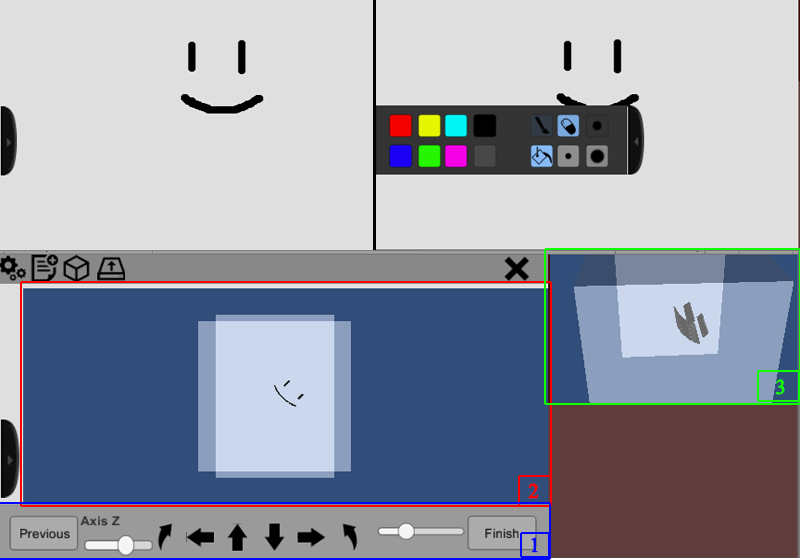
\includegraphics[scale=0.5]{images/Cmt_placer.png}}
		
		Une fois le dessin extrudé, pour le placer dans l'environnement 3D, l'utilisateur pourra à l'aide d'un menu (1) orienté et redimensionné la figure selon chacun de ses axes les un après les autres. Pour se retrouver dans l'environnement, il aura une caméra qui suit l'objet selon l'axe courant (2). Et une caméra amovible et zoomable qui filmera l'ensemble de la scène déjà créée (3). Ici les cubes sont des objets créés précédemment qui sont passés en transparent pour faciliter la lisibilité.\newline\newline

		Une fois tout ces points définis , nous avons pu passer à l'étape suivante, c'est-à-dire l'architecture du logiciel.
		
	\section{Architecture logicielle}
		Nous avons découpé le logiciel en plusieurs sous parties qui peuvent être développer indépendamment. Les liens entre les parties obligent à crée des fonctions qui envoie certaines données. L'avantage de cette découpe est qu'une étape est en majorité indépendante de la précédente. Donc on peut développer et tester chaque partie de façon optimiser avant de tout réunir et lié.
		
		Nous avons omis dans le schéma la caméra de prévisualisation, elle est contenu dans
		'Objet', qui représente l'assemblage des divers dessins 2D extrudés.

				\centerline{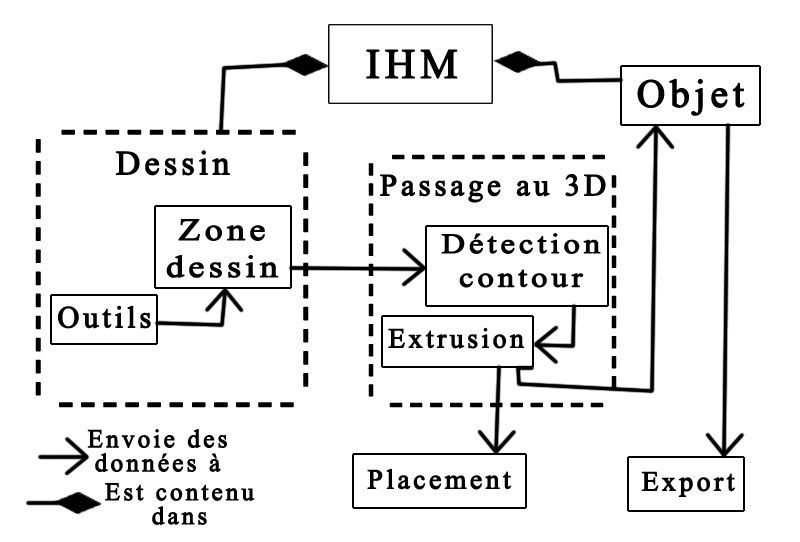
\includegraphics[scale=0.5]{images/archi.png}}


	\section{Etape par étape}
		%combien de temps passé pour chaque tâche
		%Problèmes rencontrées et solutions apportées, en quoi ces solutions ont été utilisées par la suite
		\subsection{L'IHM}
			La difficulté de la création de l'Interface Homme-Machine (IHM) étais de concevoir un espace ergonomique et adapté pour recevoir le reste des éléments de l'application. Après une conception sur papier pour assurer l'adaptabilité, nous avant développer cela avec des outils récemment intégré à Unity, les 'UI', ils sont dédiés à la création de fenêtres et de menus. Leur utilisation limite la production de code de notre part et permet une gestion plus optimisé de ces éléments.
			
			Voici donc l'IHM finale, avec une zone de dessins (1) et qui servira pour le placement, une barre d'outils (2), une zone pour la prévisualisation (3) et une dernière pour la possible future gestion des figures créée (4).
			
			\centerline{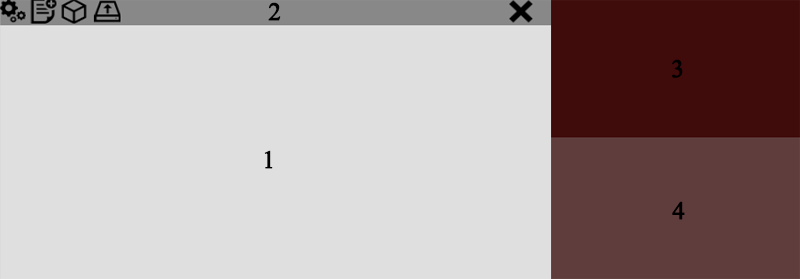
\includegraphics[scale=0.5]{images/ihm.png}}

			Chaque boutons ouvrent sur des fenêtres qui n'attendent plus que la liaisons avec les fonctions des autres sections de l'application.
			
			Pour respecter la propriété intellectuelle, nous avons dessiné une partie des boutons et pris une autre sur iconmonstr.com (un site proposant des icônes libres pour notre utilisation).
		\subsection{Dessin}
		
			\subsubsection{Outils}	
						
				Les outils sont dans un menu coulissant, pour animé le mouvement, un outils est intégré dans Unity, les animations. Nous avons accéléré ces animations après de tests utilisateurs.
					
				Pour permettre à un utilisateur novice d'utiliser l'application, nous avons proposer à l'utilisateur un nombre limiter d'outils, de couleurs et de diamètres. On aurai pu être plus exhaustif, avec par exemple un choix des quantités de chaque couleurs primaires entre 1 et 255 pour couvrir toute la palette chromatique. Mais cela aurai trop complexifié l'application.
				Dans cette partie il est très facile d'ajouté des outils ou couleurs sans toucher au reste du programme. Il n'y as qu'une fonction a écrire et le canevas de ces fonctions est déjà présent dans le code.
			\subsubsection{Zone dessin}
			
			C'est pour nous la première étape de la création d'un objet 3D. À la suite de cette étape, nous souhaitions obtenir une image à extruder. Les images sont appelées textures sous Unity. Nous avons utilisé un plan comme objet de référence pour la zone de dessin. Nous nous sommes rendus compte plus tard que la texture de base ne prenait pas l'alpha\footnote{C'est à dire la transparence} en compte, or nous souhaitions disposer d'une image où seul les parties coloriées seraient extrudées. Nous avons donc précisé, lors de la création de la texture, vouloir un type RGB32, pour avoir un fond transparent.
			
			Un premier problème apparut alors quant au dimensionnement de cette zone de dessin. Le plan ayant une taille précise, il fallait être capable de modifier sa taille par rapport à celle du canevas. Nous avons donc rédigé un script qui initialise la dimension de la zone de dessin, autant pour le plan que pour la texture qui lui est associée.
			
			Le dessin se trace sur la texture à l'endroit où l'on clique. Or nous ne pouvions pas juste utiliser la position du curseur, car les dimensions de la texture sont indépendantes et s'adaptent de celle de l'objet. Un moyen efficace pour modifier la texture en cliquant sur l'objet est de projeter un Ray, objet monodirectionnel qui traverse l'espace, au moment où l'on clique dans la zone de dessin, et de trouver le pixel à l'intersection de ces deux objets. Nous avons ainsi pu, dans un premier temps, modifier un pixel en cliquant dessus. Ensuite, pour garder un tracé continu, nous avons implémenté une méthode qui trace la droite entre le dernier point colorié, et le point sur lequel on clique. Pour cela, nous utilisons l'équation cartésienne de la droite :
			\centerline{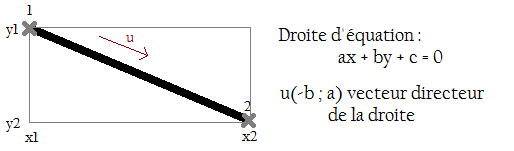
\includegraphics[scale=0.6]{images/trait.png}}
			Ensuite, nous observons les pixels contenus dans ce cadre augmenté de la largeur du trait pour ne pas en perdre dans les coins, ou quand le trait est quasi droit. Les pixels dont la distance à la droite est inférieure à la largeur du trait sont coloriés.
			
			 Il restait à faire le lien entre la zone de dessin, et les différents outils définis plus tôt. Ainsi, la zone de dessin va chercher les différentes couleurs, la largeur du trait, et les outils à utiliser dans le menu déroulant. Nous avons aussi implémenté des méthodes "eraser" et "bucket", capables de gommer et remplir rapidement une surface. Pour le bucket, nous avons utilisé un algorithme classique de remplissage par diffusion avec une pile explicite\footnote{http://fr.wikipedia.org/wiki/Algorithme\_de\_remplissage\_par\_diffusion}.
			
		\hypertarget{ancre}{
		\subsection{Passage au 3D}}
		\label{extrusion}
		L'extrusion est une autre tâche importante du projet. En effet, il faut à partir d'une texture, créer un objet en 3D. Pour ce faire, nous sommes partis d'une extension Unity déjà existante : UCLA Mesh Creator. C'est un créateur d'objets 3D, à partir d'une texture. Seulement, il a fallu reprendre le code pour l'adapter à notre utilisation. Initialement, cette application sert à créer rapidement et simplement un objet afin de pouvoir l'insérer dans son jeu. De plus, il est possible de la faire fonctionner uniquement en mode "édition". Il y a deux modes quand on l'on travaille sous Unity : le mode "édition", qui nous permet de créer des scènes avec nos objets, nos animations, et un mode "jeu" où l'on voit le rendu final avec lequel l'utilisateur interagira. Nous nous sommes donc concentrés sur l'adaptation du code déjà existant plutôt que sur la recherche et l'implémentation d'un ou plusieurs algorithmes afin de détecter les contours d'une image. Seulement, comme c'est une adaptation, il y a eu une longue phase de compréhension et de test afin de faire fonctionner comme il faut cette application. 
		\subsection{Placement et prévisualisation}
		
			Pour placer l'objet courant, nous avons juste intégré des scripts qui translate la figure et des sliders pour choisir la taille. La vitesse et rotation/translation et les tailles admises par les figures sont facilement modifiables, elles nécessiteront probablement des ajustements. Ou sinon un traitement de l'objet dans le serveur peut être imaginer, où celui-ci augmenterai la taille de l'objet pour l'adapter à la salle de réalité augmenté.
			
			Pour la prévisualisation et le placement, nous avons intégré des caméras. Celles-ci sont adapté aux objets créée. Mais si on ajuste les tailles des objets, il faudrait aussi modifier la taille de ces caméras.

		\subsection{Export}
			Un fois l'objet en 3D créé, nous devons l'envoyer à un serveur qui affichera cet objet dans une scène 3D.
			Nous nous sommes orientés vers le socket TCP qui permet d'échanger des données entre 2 applications.
			Nous avons choisi cette approche de l'envoi des données car:
			\begin{itemize}
				\item Elle dispose de classes prévues à cet effet en C\#
				\item Elle est documentée en C\# par Microsoft
				\item Elle permet d'envoyer des octets, donc flexible
			\end{itemize}
						
			
			\centerline{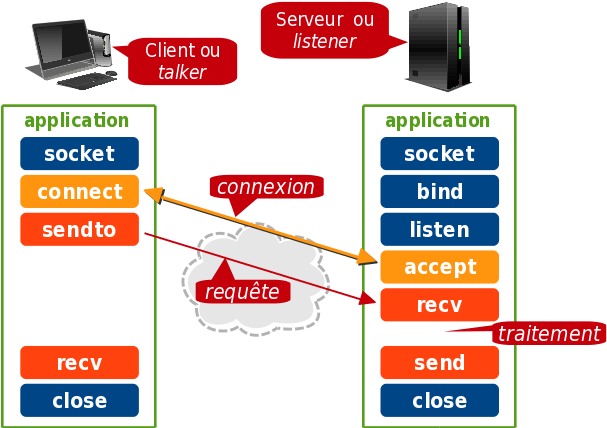
\includegraphics[scale=1]{images/tcp-socket.png}}
			
			Dès que la connexion est établie, le client envoie sous forme de flux les données de l'objet en 3D. Cette action correspond à la requête sur le schéma. Puis, en guise de traitement, le serveur affiche l'objet en 3D dans la scène.
			Dans notre cas, un script léger du côté du serveur permet de gérer la connexion avec le client et l'affichage de l'objet.
			
	\section{Organisation du travail}
				
				Pour réalisé toutes ces tâches en parallèles, nous avons hébergé notre projet sous GitHub. La répartition des tâches fut comme suis:
				- Aurélien Fontaine : Passage au 3D
				- Etienne Geantet : Zone Dessin
				- Manutea Huang : Export
				- Arnaud Martin : IHM - Outils - Placement - Prévisualisation
			
				Nous n'avons pas rencontrer de problème lors de la mise en commun des parties. A part au niveau du passage de la texture de la zone de dessin à l'extrusion:
				%je vous laisse expliquer
			
				Afin de faire un point régulier et d'être sûr de répondre aux exigences de notre encadrant, nous nous sommes réunis hebdomadairement. Au cours de ces séances, nous pouvions ainsi voir le travail effectué par les différents membres de notre projet et nous pouvions bénéficier de l'expérience de M. François LEHERICEY avec Unity.
				
				Cette organisation du travail c'est majoritairement révélé efficace. Nous aurions dû fixer notre choix sur Unity dés Octobre et passer moins de temps sur l'état de l'art pour le choix du logiciel. cela nous aurai permis de faire des recherches plus ciblé et ainsi trouver Ucla Mesh Creator plus tôt. De plus nous aurions pu commencer à acquérir des connaissances basiques sur Unity. Manque de connaissance qui nous a ralenti.
			
	
	\section{Objectifs}
		%Qu'est-ce qu'on a : changé, abandonné ...

	%	Pour le dessin, nous nous sommes contenté de trois tailles pour l'outil de coloriage.
	%	La possibilité de sauvegarder des objets n'était pas, à l'origine, une des fonctionnalités de l'application. Mais en se concertant, nous nous sommes rendu compte qu'une personne aimerait sûrement pouvoir réutiliser ses objets dans la construction d'autres objets. Si toutes les autres fonctionnalités de l'application sont opérationnelles, la sauvegarde serait un objectif potentiel à rajouter.
	%	Globalement, nous sommes arrivés à un résultat très proche de notre conception initiale de l'application.Notre application a encore plusieurs voies d'améliorations possibles. Comme l'implantation d'outils pour faire des sphères, avec des extrusions circulaires.
		Au cours de l'avancement du projet, nous avons du faire certains choix, et changer ou abandonner certaines de nos idées initiales. Notamment : la sauvegarde et l'éditions des éléments créées.
		Par manque de temps nous n'avons pas pu les implantés nous même, mais dans l'IHM des menus sont déjà présents pour géré la sauvegarde et nous savons en théorie comment mettre en place la liste d'objet, tout cela sera intégré dans la documentation utilisateur.
		Globalement, nous sommes arrivés à un résultat très proche de notre conception initiale de l'application et qui répond au cahier des charges.
	
	\section{Conclusion}
		%Ce que l'on se souviendra du projet
		%Si c'était à refaire, quoi changer?
		%Quelles sont les évolutions que l'on pourrait apporter à notre application finale
		%	Nous en retenons qu'Unity est un outil puissant, mais pas encore adapté à la création de menus, et orienté pair-à-pair. Ce travail fut aussi une bonne initiation à la gestion de projet, avec l'utilisation de Git. Il en ressort aussi qu'il est crucial de se donner des tâches précises et des délais à respecter pour arriver au bout d'un projet dans les temps impartis. Cela évite qu'une partie minime du projet ne nous accapare tout notre temps.
			
		%	Si l'on nous présentait ce projet à nouveau, nous changerions notre méthode de travail sur plusieurs points. Notamment, nous passerions moins de temps sur l'état de l'art; il était presque sûr qu'Unity serait notre choix comme outil de développement. Ensuite, nous procéderions à un partage des recherches et des réflexions aux premiers instants du projet. Nous commencerions à apprendre à utiliser Unity dès le mois d'Octobre, car ce manque de connaissances nous a relenti par la suite. Nous étions parfois bloqués par des détails, ou nous trouvions des solutions sans les comprendre entièrement, menant à d'autres problèmes par la suite. Mais le manque de temps ne nous permettait pas de faire autrement.
		Nous avons atteint les objectifs du cahier des charges:
		L'application est donc utilisable sur tablette Windows, possède une interface graphique, une gestion du dessin, une extrusion avec prévisualisation et enfin un mode de transfert de l'objet 3D. L'utilisation de Unity, un logiciel puissant et évoluant, assure un suivi et de possibles évolutions facilitées par l'application.
		
		Nous avons réalisé des tests avec des utilisateurs, ce qui assure un certain niveau d'ergonomie. En précisant juste où se trouve les outils et le menu extrudés, ils arrivent à créer des objets 3D.
		
		L'utilisation d'un système de gestion de version est un vrai plus dans un projet de groupe, il faut garder à l'esprit que nous réflechissons tous différemment: il est primordial de bien définir les règles qui permettent de lier les différentes fonctionnalités de l'application.
		

	
	\section{Remerciements}
		Nous souhaitons tout d'abord remercier Monsieur François LEHERICEY pour sa disponibilité ainsi que pour ses précieuses informations.
		
		Nous voudrions également remercier Monsieur Bertrand COUASNON pour son apport de connaissances ainsi que son aide dans l'élaboration de nos différentes présentations.
	
\end{document}